\section{Graph databases}
\label{sec:graphdb}
A graph database management system (graph database) \citep{robinson13} is a database management system based on graph theory. The term graph theory has been used in centuries and was first introduced by the Swiss mathematician Leonard Euler (1707-1783). In 1736, he proved that there does not exist a closed walk that crossed exactly once each of the seven bridges of the river Pregel in Köningsberg, now called Kaliningrad \citep{alexanderson06}. Figure \vref{fig:7bridgesEuler} shows Euler's original drawings from his paper written in 1736 \citep{euler1741} of the bridges in Köningsberg. 

\begin{figure}[H]
  \centering
  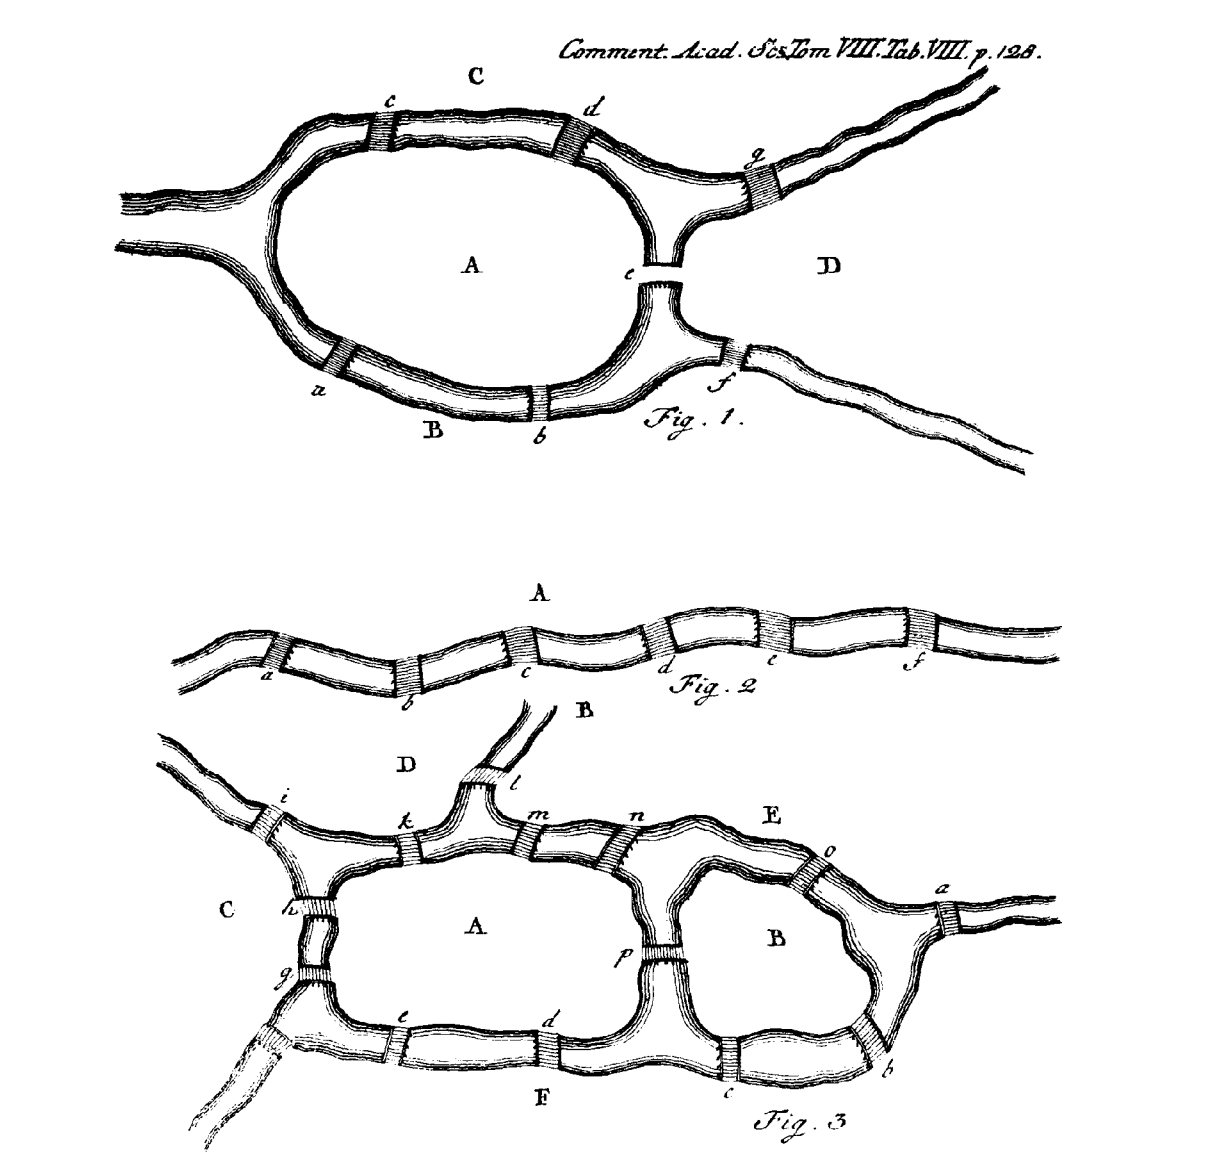
\includegraphics[width=3in]{assets/7bridges-euler.png}
  \caption{Eulers original drawing of the Seven Bridges of Köningsberg} 
  \label{fig:7bridgesEuler}
\end{figure}

%Based on the solution of the ``Seven Bridges of Köningsberg''-problem, Euler presented a theorem. This theorem states that if the graph is planar and connected, and if \textit{v} is the number of vertices, \textit{e} is the number of edges and \textit{f} is the number of faces\footnote{Regions between edges of a plane graph that does not have any edges in it}, then 
%\newline
%\newline
%\centerline{$v-e+f=2$}
%\newline
%\newline
%This theorem demonstrates that if it does not exist a path in the graph that will allow to visit every node using every edge exactly once, the sum will not be 2. An illustration of the bridges in Köningsberg as a graph is presented Figure \vref{fig:7bridgesIllustration} and simplified the illustration in figure \vref{fig:7bridgesSimplification}. The graph consists of 4 vertices, seven edges, and four faces, where the faces are specified with numbers 1-4. If the theorem described above is used, we see that $4-7+4\neq2$, which is consistent with Euler's proof from 1736. 

%\begin{figure}[H]
%  \centering
%  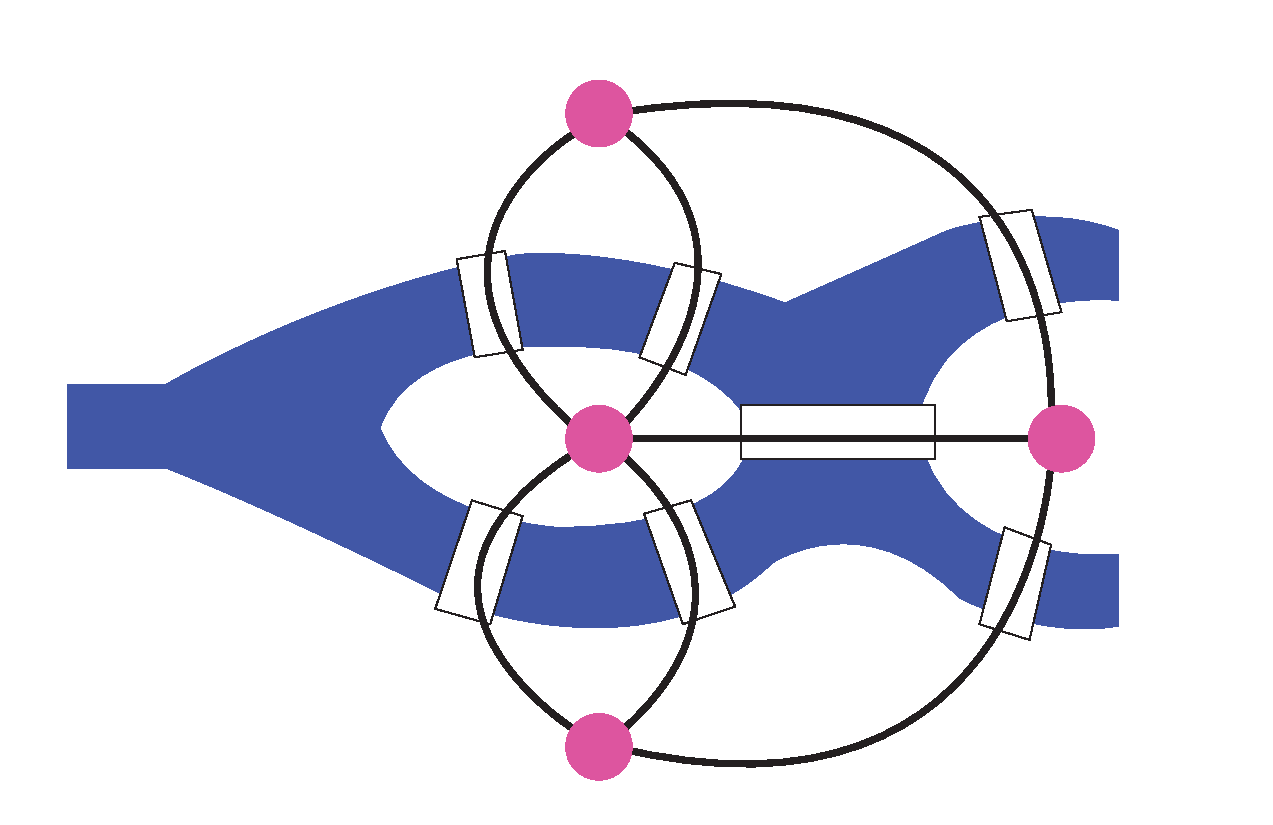
\includegraphics[width=4in]{assets/7bridges.pdf}
%  \caption{Illustration of the Seven Bridges of Köningsberg as a graph}
%  \label{fig:7bridgesIllustration}
%\end{figure}

%\begin{figure}[H]
%  \centering
%  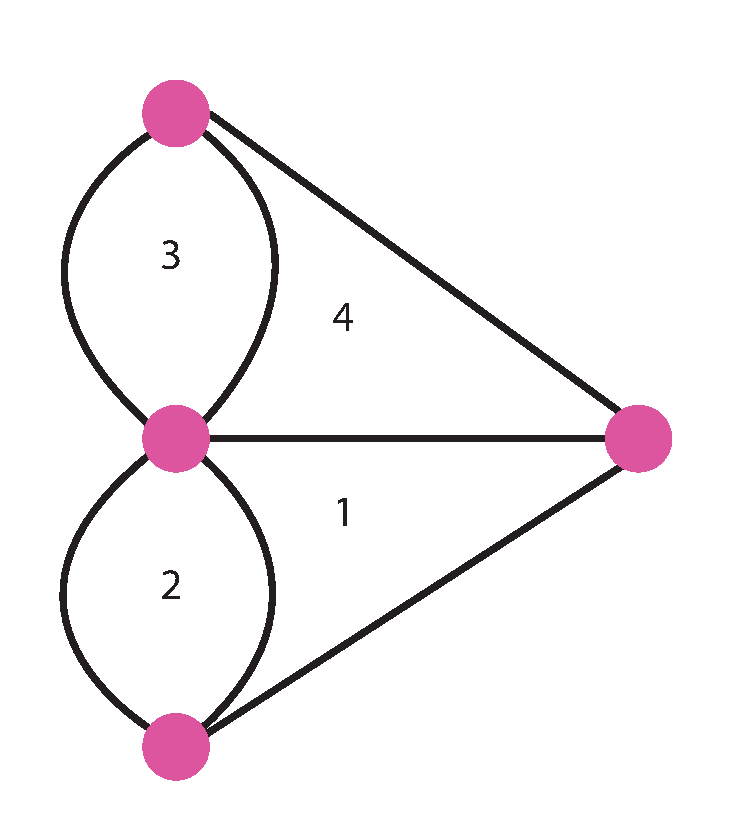
\includegraphics[width=2in]{assets/7bridges2.pdf}
%  \caption{Illustration of the Seven Bridges of Köningsberg as a simplified graph} 
%  \label{fig:7bridgesSimplification}
%\end{figure}

Graph databases use graph structures for semantic queries with nodes, edges, and properties to represent and store data.
The nodes represent entities, such as people, accounts, or bus stops, while the edges represent the relationships, such as ``Friend of'' or ``Belongs to'', between the nodes. A property is relevant information that can relate to either a node or an edge, such as ``Name'' or ``Travel Time''.
%Må omformuleres
Applications of graph databases can include calculating routes and finding the shortest path between locations in a network, such as a road or rail network, airspace network, or logistical network \citep[p.102]{robinson13}. 
%Må omformuleres Compared to relational databases, are graph databases often faster for associative data sets, and map more directly to the structure of object-oriented applications. They can scale more naturally to large data sets as they do not typically require extensive join operations. A drawback to graph databases is the inertia of finding all objects of a specific type.  The following operations are not recommended using graph databases: large, set-oriented wueries, graph global operations and simple, aggregate-oriented queries\citep[p. 40-41]{bruggen14}

\subsection{Neo4j}
\label{subsubsec:neo4j}
Neo4j \citep{website:neo4j} is an open-source graph database, implemented in Java. It is ranked the most popular graph database worldwide \citep{website:graphdbranking} and is used by several large companies such as Telenor \citep{website:telenor}, Walmart \citep{website:walmart} and Cisco \citep{website:cisco}. It is a native graph database optimized and designed for storing and managing graphs and is known for extremely fast traversals of relationship. The underlying data model of Neo4j is the labeled property graph and is one of the most generic and versatile of all graph models \citep[p.73]{robinson13}. This graph data model gives four different fundamental building blocks to structure and store data. These building blocks includes Nodes to store entity information, Relationships to connect nodes to another, Properties for relevant information, and Labels for creating subgraphs.

A query that is extremely well suited for graph databases are queries for finding the paths between different nodes in a graph. Neo4j can be used to see whether a path exists, finding the optimal path, and looking for variability in the path \citep[p. 51]{bruggen14}. Neo4j includes built-in methods for finding the shortest path, including Dijkstra's algorithm. Dijkstra's algorithm \citep[p.658-662]{cormen09} maintains a set $S$ of vertices' whose final shortest-path weights from the source $s$ have already been determined. The algorithm repeatedly selects the vertex $u = V - S$ with the minimum shortest path estimate, adds $u$ to $S$, and relaxes\footnote{Making a change that reduces constraints.} all edges leaving $u$. The running time of Dijkstra's algorithm is $O((V + E)log V)$ and it is guaranteed to find the shortest path \citep[p.~661]{cormen09}. %Dijkstra is one of the best-known algorithms to calculate the shortest weighted path between two points on a graph, using the properties of the edges as a weight or costs. 
The Relationships in a Neo4j database are capable of being of different RelationshipTypes that, among others, enables the built-in Dijkstra to find the shortest path using only specific RelationshipTypes.

%Sweet spot use cases of neo4j: complex, join-intensive queries, path finding queries\citep[p. 51]{bruggen14}. 

%TODO skrive mer her

%Advantages:
%\begin{itemize} 
%\item Flexibility: model, develop and visualize the world as you experience it. Its simply nodes and relationships. 
%\item Performance: Hyper-connectivity at speed. 
%\item Scalability: Scales up and out, supporting tens of billions of nodes and relationships, and hundred of thousands of ACID transactions per seconds. 
%\item Speed: Able to search trough millions of connections per second, with real time queries that stay fast even as your database grows. 
%\end{itemize}

%\begin{itemize}
%\item Native graph database. 
%\item Property graph. 
%\item Made for real time queries. 
%\item Really fast traversals of relations.
%\item Neo4J has an API that supports traversing - finding shortest path - can weight edges, nodes -
%\end{itemize}
%//en korteste vei mellom n og m men max lengde 3
%match p = shortestPath ( (n) - [*...3]--(m)) return p
%(Vekte kanter: Neo44J har et API som støtter traversering, Dijkstras er innebyd ++ som lar deg vekte kanter - hva er raskeste vei ++)

%Neo4J can be used to evaluate routes after the ants have created route sets.